\documentclass[CJK,11pt]{amsart}
\usepackage{CJK}
\usepackage{lipsum}
\usepackage{amsfonts}
\usepackage{graphicx}
\usepackage{epstopdf}
\usepackage{algorithmic}
\usepackage{hyperref}
\hypersetup{
	colorlinks=true,
	linkcolor=blue,
	filecolor=blue,      
	urlcolor=blue,
	citecolor=cyan,
}
\ifpdf
  \DeclareGraphicsExtensions{.eps,.pdf,.png,.jpg}
\else
  \DeclareGraphicsExtensions{.eps}
\fi

% Add a serial/Oxford comma by default.
\newcommand{\creflastconjunction}{, and~}

\usepackage{amsopn}
\DeclareMathOperator{\diag}{diag}

\usepackage{relsize}
\usepackage{pxfonts}
\usepackage{tikz}
\usetikzlibrary{arrows,shapes,chains,positioning}
\usetikzlibrary{decorations.markings}
\tikzstyle arrowstyle=[scale=1]
\tikzstyle directed=[postaction={decorate,decoration={markings,mark=at position .65 with {\arrow[arrowstyle]{stealth}}}}]
\tikzstyle reverse directed=[postaction={decorate,decoration={markings,mark=at position .65 with {\arrowreversed[arrowstyle]{stealth};}}}]
\newtheorem{Def}{Definition}
\newtheorem{Th}{Theorem}[section]
\newtheorem{Lm}{Lemma}[section] 
  
\theoremstyle{definition}
\begin{document}
\begin{CJK*}{UTF8}{gbsn}
\title{
The Life and Mathematics of James H. Bramble
}
\author{Students of Bramble}
\maketitle

\section{News and family}
James Henry Bramble, one of the most distinguished computational mathematicians of all times and our beloved mentor and friend, died July 20, 2021 at his home in Austin, Texas. He was 90.

Bramble was born on December 1, 1930 in Annapolis, Maryland to Edith and Clinton Bramble. He had two sisters, Mary Aller and Barbara Lawrence, both deceased. 
In 1978, Bramble married Margaret (Peggy) Hays, now deceased (when???). 
He is survived by his four children, Margot Dermody of Pittsburgh, Pennsylvania, Tamara Lamenzo of Needham, Massachusetts, Mitzi Bramble of Harwich, Massachusetts, and James Bramble of Austin, his step-son, Alan Hays of Ithaca, and eight grand-children. He also is survived by his first wife, Mary Eppie Boze. 

He earned his bachelor degree from Brown University in 1953,  a master degree and Ph.D. degree from the University of Maryland in 1955 and 1958 respectively. He then worked for General Electric, the Naval Ordnance Laboratory and the University of Maryland. In 1968, he was recruited to Cornell.  

After working for General Electric and the Naval Ordnance Laboratory, he became a professor at the University of Maryland and then at Cornell University

After retiring from Cornell 1994 and then retiring from Texas A\&M in ????, Bramble and his wife, Peggy, remained in Austin, but returned to their lakeside cottage in Ithaca every summer. 
They enjoyed entertaining friends and family, playing golf and tennis, and boating.

He will be remembered fondly by family, friends, and colleagues worldwide

\subsection{Cornell days}
In his 26 years at Cornell, as professor of mathematics in the College of Arts and Sciences,  Bramble helped move his department to the forefront of applied mathematics and became a leading figure in his field, bridging rigorous theory and practical numerical computation.  “Cornell hired Professor Bramble to help establish a world-class group in numerical analysis,” said Tara Holm, professor of mathematics and department chair. “That group began with his adviser, Larry Payne, and later included professors Lars Wahlbin and Al Schatz. Bramble was one of the top three in his field in the country and of worldwide renown. He put applied mathematics at Cornell on the world map, as it were. Bramble’s work remains central in applied mathematics and continues to be highly cited today.”

Bramble also made a significant impact with Cornell’s Center for Applied Mathematics. He served as its director from 1975-81, helping to secure university funding for graduate students.  In addition, Bramble served as associate chair and director of undergraduate studies in the Department of Mathematics for three years, and as graduate faculty representative in mathematics for three years.  Holm said.

\subsection{Texas A\&M}
In 1994, he retired from Cornell as professor emeritus. He continued his career at Texas A\&M University, where he retired in (when ????) as Distinguished Professor Emeritus. 

He was an editor at the journal {\it Mathematics of Computation} for 25 years, and chief editor from 1975-83. He received an honorary doctorate from Chalmers University of Technology in Sweden in 1985.  in recognition of his important contributions to mathematics.

In 1970, along with Ivo Babuska and Bruce Kellog, Bramble co-founded the Finite Element Circus (https://sites.google.com/view/fecircus), a regular meeting devoted to the theory and applications of the finite element method and related areas of numerical analysis and partial differential equations.  In the early years meetings were held as often as four times a year, but soon a format was established of a one-and-one-half day meeting held every spring and fall at varying locations.  The Finite Element Circus has played a critical role in making the finite element method as one of the major numerical methods for solving partial differential equations, and in training generations of researchers in finite element method.

\subsection{Ph.D. students of Bramble}
Bramble taught numerous undergraduate and graduate students, mentored 22 PhD students, and had colleagues throughout the world. Here is a list:
% Selina help with this file
\begin{enumerate}
\item \href{https://www.linkedin.com/in/maxine-rockoff-394b114/}{Maxine Rockoff}(University of Pennsylvania, 1964), currently an adjunct associate research scientist at Columbia University.
\item \href{http://euclid.colorado.edu/~gustafs/}{Karl Gustafson}(University of Pennsylvania, 1965), currently a professor of mathematics at University of Colorado Boulder.
\item \href{https://cs.uwaterloo.ca/~rbsimpso/RBScv.pdf}{Richard Bruce Simpson}(University of Maryland, 1966), used to be a professor of computer science at uniersity of Waterloo, passed away in 2020.
\item \href{https://ep.jhu.edu/faculty/james-kuttler/}{James Kuttler}(University of Maryland, 1967), currently an instructor in JHU Whiting School of Engineering.
\item \href{https://en.wikipedia.org/wiki/Stephen_Hilbert}{Stephan Hilbert}(University of Maryland, 1969), used to be a professor of mathematics at Ithaca College.
\item \href{https://sites.math.rutgers.edu/~falk/}{Richard Falk}(Cornell University, 1971), currently a professor of mathematics at Rutgers.
\item Thomas King(Cornell University, 1971).
\item \href{https://www.legacy.com/us/obituaries/knoxnews/name/steven-serbin-obituary?pid=120620923}{Steven Serbin}(Cornell University, 1971), used to be a professor of mathematics at University of Tennessee, passed away in 2008.
\item \href{http://www.math.buffalo.edu/mad/PEEPS/baker_gartha.html}{Garth Baker}(Cornell University, 1973), used to be a lecturer of mathematics at Bermuda College.
\item \href{https://services.math.duke.edu/~johnt/}{John Trangenstein}(Cornell University, 1975), currently a professor of mathematics at Duke University.
\item \href{https://www.math.tamu.edu/~joe.pasciak/}{Joseph E. Pasciak}(Cornell University, 1977), currently a professor of mathematics at Texas A\&M University.
\item \href{https://www.mn.uio.no/math/english/people/aca/rwinther/}{Ragnar Winther}(Cornell University, 1977), currently a professor of mathematics at University of OSLO.
\item Peter Sammon(Cornell University, 1978).
\item \href{https://www.uah.edu/science/departments/math/faculty-staff/mark-pekker}{Mark J. Pekker}(Cornell University, 1982), currently a professor of mathematics at The University of Alabama in Huntsville.
\item \href{https://www.personal.psu.edu/jxx1/}{Jinchao Xu}(Cornell University, 1989), currently a professor of mathematics at Pennsylvania State University. 
\item Ping Lee(Cornell University, 1990).
\item Mark Hanisch(Cornell University, 1991).
\item \href{https://www.bgsu.edu/arts-and-sciences/mathematics-and-statistics/faculty-and-staff/tong-sun.html}{Tong Sun}(Texas A\&M, 1997), currently a professor of mathematics at Bowling Green State University.
\item \href{http://web.pdx.edu/~gjay/}{Jay Gopalakrishnan}(Texas A\&M, 1999), currently a professor of mathematics at Portland State University.
\item \href{http://www.math.udel.edu/~bacuta/}{Constantin Bacuta}(Texas A\&M, 2000), currently a professor of mathematics at University of Delaware.
\item \href{https://people.llnl.gov/kolev1}{Tzanio Kolev}(Texas A\&M, 2004), currently a computational mathematician at Lawrence Livermore National Laboratory.
\item \href{https://scholar.google.com/citations?user=EeWTb_wAAAAJ&hl=en}{Dimitar Trenev} (Texas A\&M, 2009), currently working at ExxonMobil Corporate Strategic Research.
\end{enumerate}


\section{Scientific contributions}


Bramble began his research career developing analytical methods for partial differential equations – that is, equations that relate functions and their derivatives.  In most of his career, 
he worked on numerical solutions of partial differential equations and multigrid method. His early work involved the mathematical analysis of finite difference methods for elliptic problems. His later work was more focused on the numerical analysis of finite element methods.  He also worked on questions concerning rapid solution of large-scale systems that result from such approximations. Such a question is: Among all the theoretically good approximations to a general class of problems, are there some that can be solved efficiently by taking advantage of modern computer architectures such as parallelism? Answers to questions like this one can bring many problems into the realm of practical feasibility. He designed approximations to solutions to problems in partial differential equations that adequately describe the problem and that can be efficiently solved using modern computing power. He was also interested in Maxwell's Equations and acoustics, including scattering problems.

A partial list of his major research interests include:
\begin{enumerate}
\item Finite difference methods
\item Finite element method
\begin{enumerate}
\item Bramble-Hilbert Lemma and error analysis
\item Super-convergence
\end{enumerate}
\item Domain decomposition methods 
\begin{enumerate}
\item Non-overlapping domain decomposition method
\item Overlapping domain decomposition method
  \end{enumerate}
\item Multigrid methods
\item PLM methods 
\end{enumerate}
\subsection{Finite difference method}
Dr. Bramble worked on the mathematical analysis of numerical methods for partial differential equations. His early work involved the mathematical analysis of finite difference methods for elliptic problems. 

In the 1960s, he helped pioneer the mathematical analysis of finite difference methods for elliptical problems. 

In a sequence of papers from 1962 to 1966, \cite{bramble1962formulation, bramble1963fourth, bramble1964finite, bramble1965finite,bramble1965approximation,bramble1966second,bramble1966error}, Bramble and collaborators had systematical studies on error analysis for finite difference methods for elliptic boundary value problems of both 2nd and 4th order with various different (Dirichlet, Neumann and mixed) boundary conditions.  For example, by discrete maximum principle, he proved that the finite difference schemes for domains with curved boundaries still have $\mathcal O(h^2)$ despite of the fact the truncation error is only of order $\mathcal (h)$ near the boundary.  As another example, in paper \cite{bramble1964finite}, he provided a special example in which case the matrix is neither diagonally dominant nor of non-negative type, but for which a maximum principle still holds. This is a deep observation of the maximum principle of finite difference methods.

%\chapter{Finite Difference Methods}

\section{On the formulation of finite difference analogues of the Dirichlet problem for Poisson's equation (1962)}
On the formulation of finite difference analogues of the Dirichlet problem for Poisson's equation \cite{bramble1962formulation}
\includepdf[pages = 2-]{Papers/FDM/bramble1962formulation.pdf}

\section{Fourth-order finite difference analogues of the Dirichlet problem for Poisson's equation in three and four dimensions (1963)}
Fourth-order finite difference analogues of the Dirichlet problem for Poisson's equation in three and four dimensions \cite{bramble1963fourth}

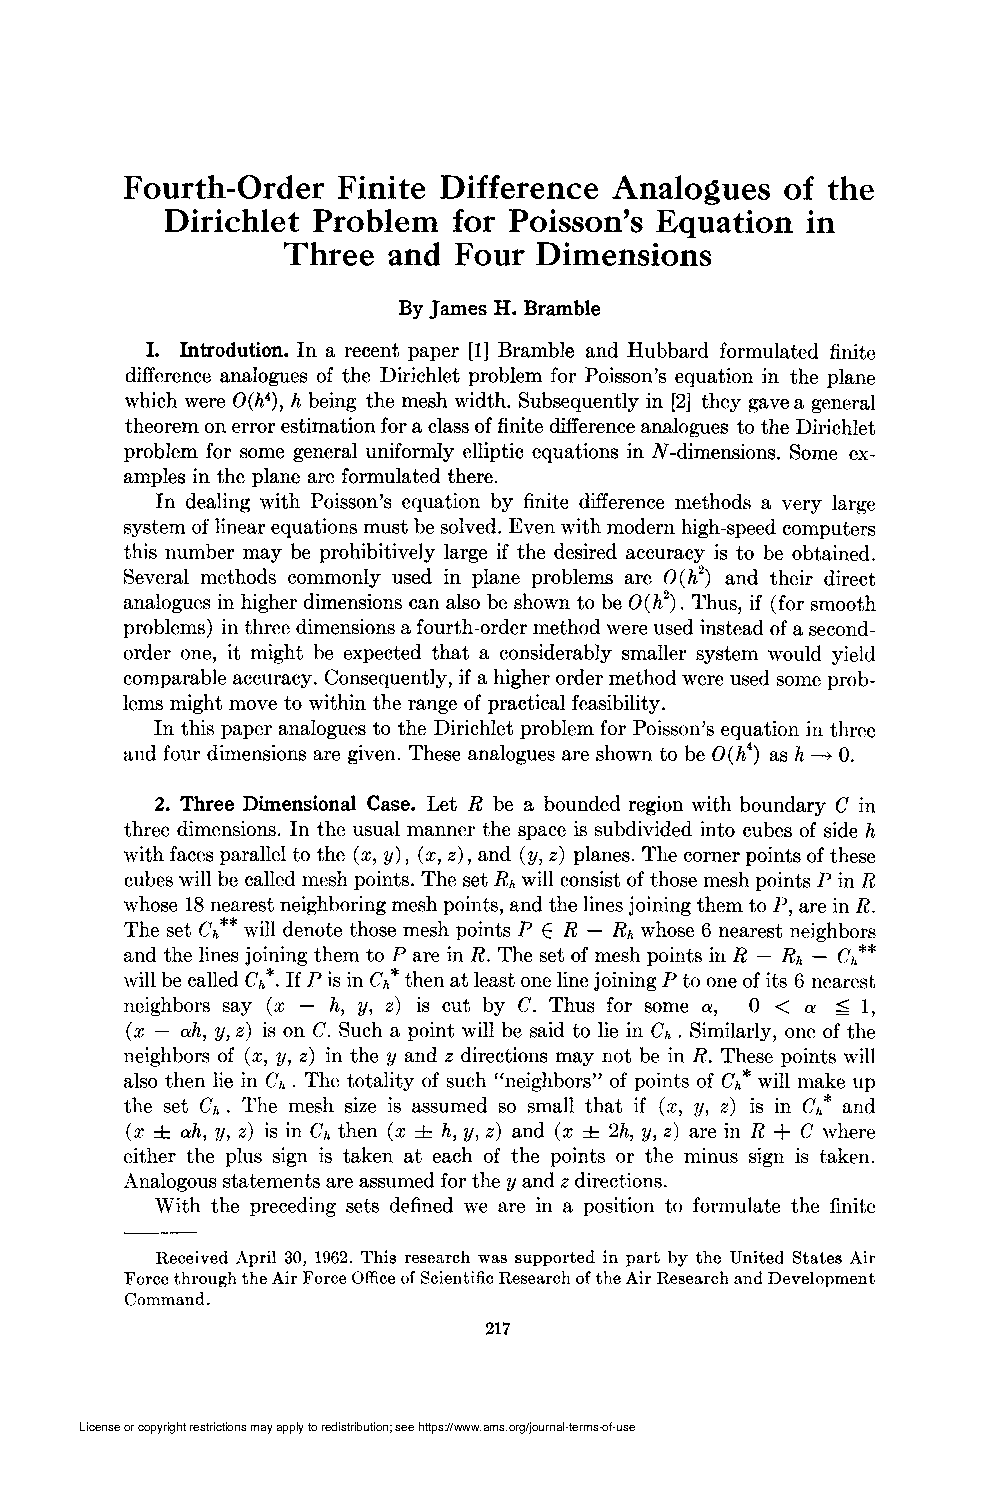
\includepdf[pages = -]{Papers/FDM/bramble1963fourth.pdf}


\section{New monotone type approximations for elliptic problems (1964)}
New monotone type approximations for elliptic problems\cite{bramble1964new}
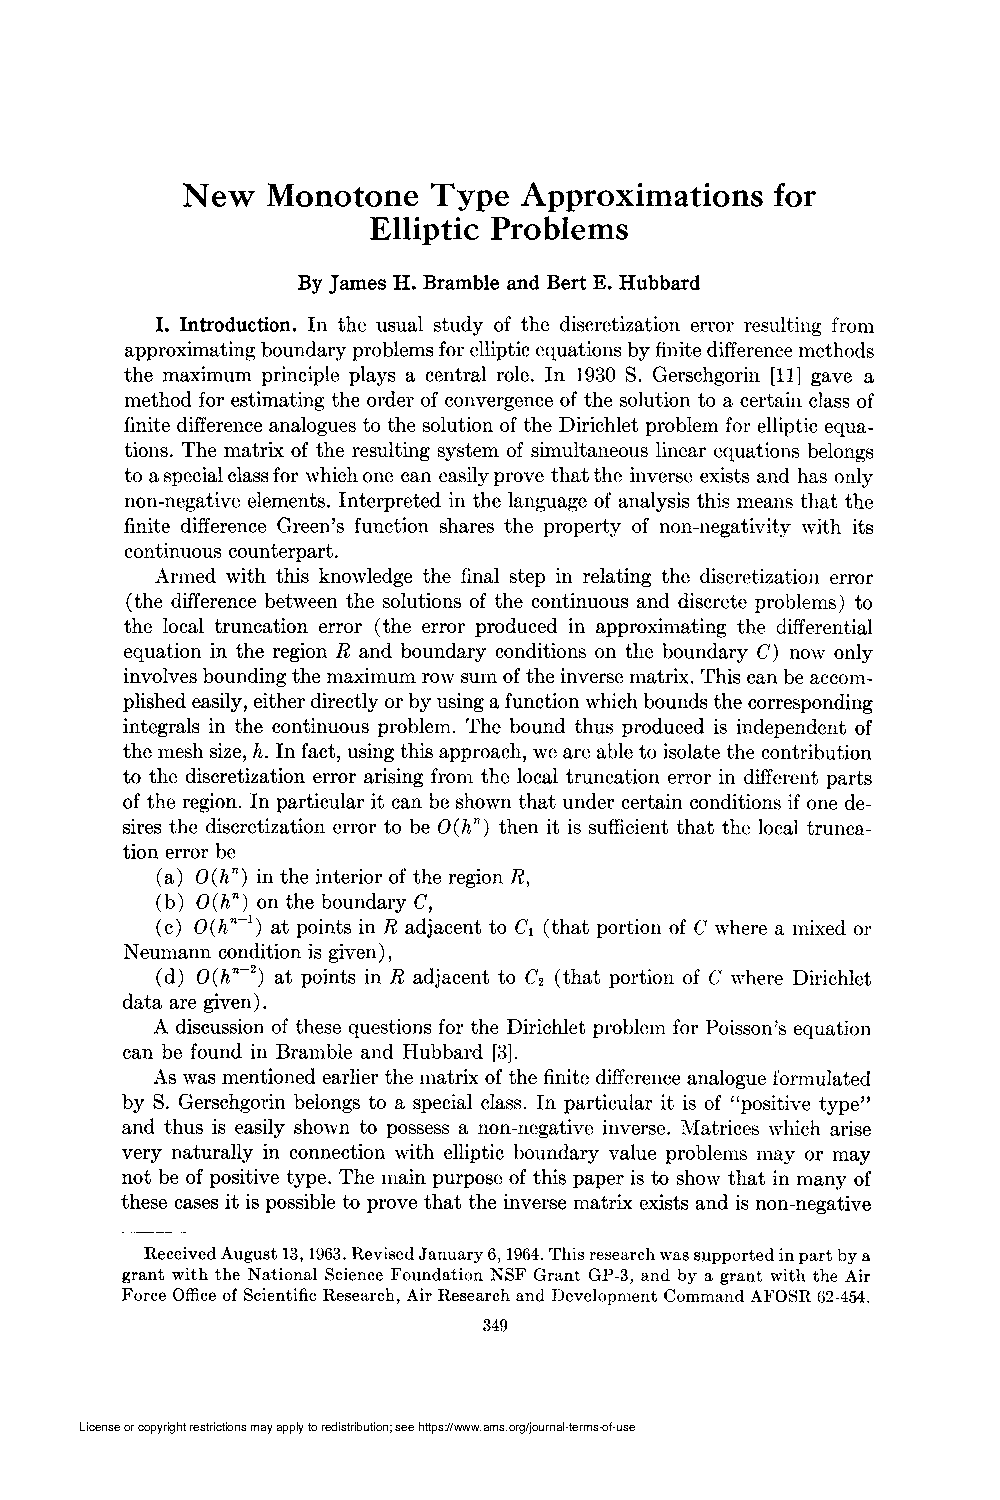
\includepdf[pages = -]{Papers/FDM/bramble1964new.pdf}

\section{On a finite difference analogue of an elliptic boundary problem which is neither diagonally dominant nor of non-negative type (1964)}

On a finite difference analogue of an elliptic boundary problem which is neither diagonally dominant nor of non-negative type \cite{bramble1964finite}

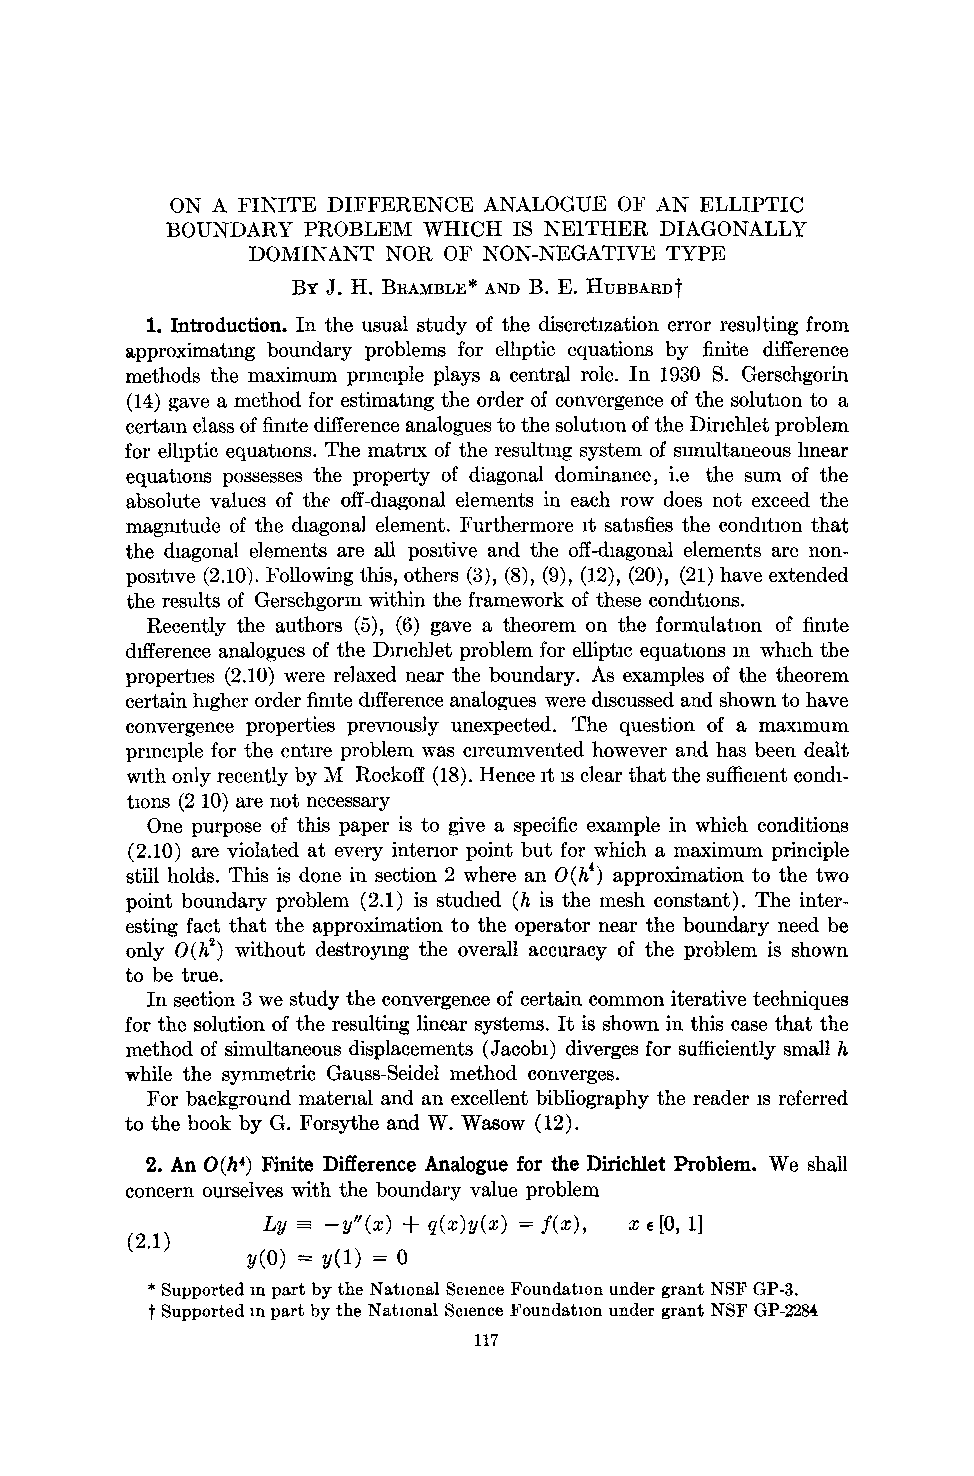
\includepdf[pages = -]{Papers/FDM/bramble1964finite.pdf}

\section{Approximation of solutions of mixed boundary value problems for Poisson's equation by finite differences (1965)}

Approximation of solutions of mixed boundary value problems for Poisson's equation by finite differences \cite{bramble1965approximation}

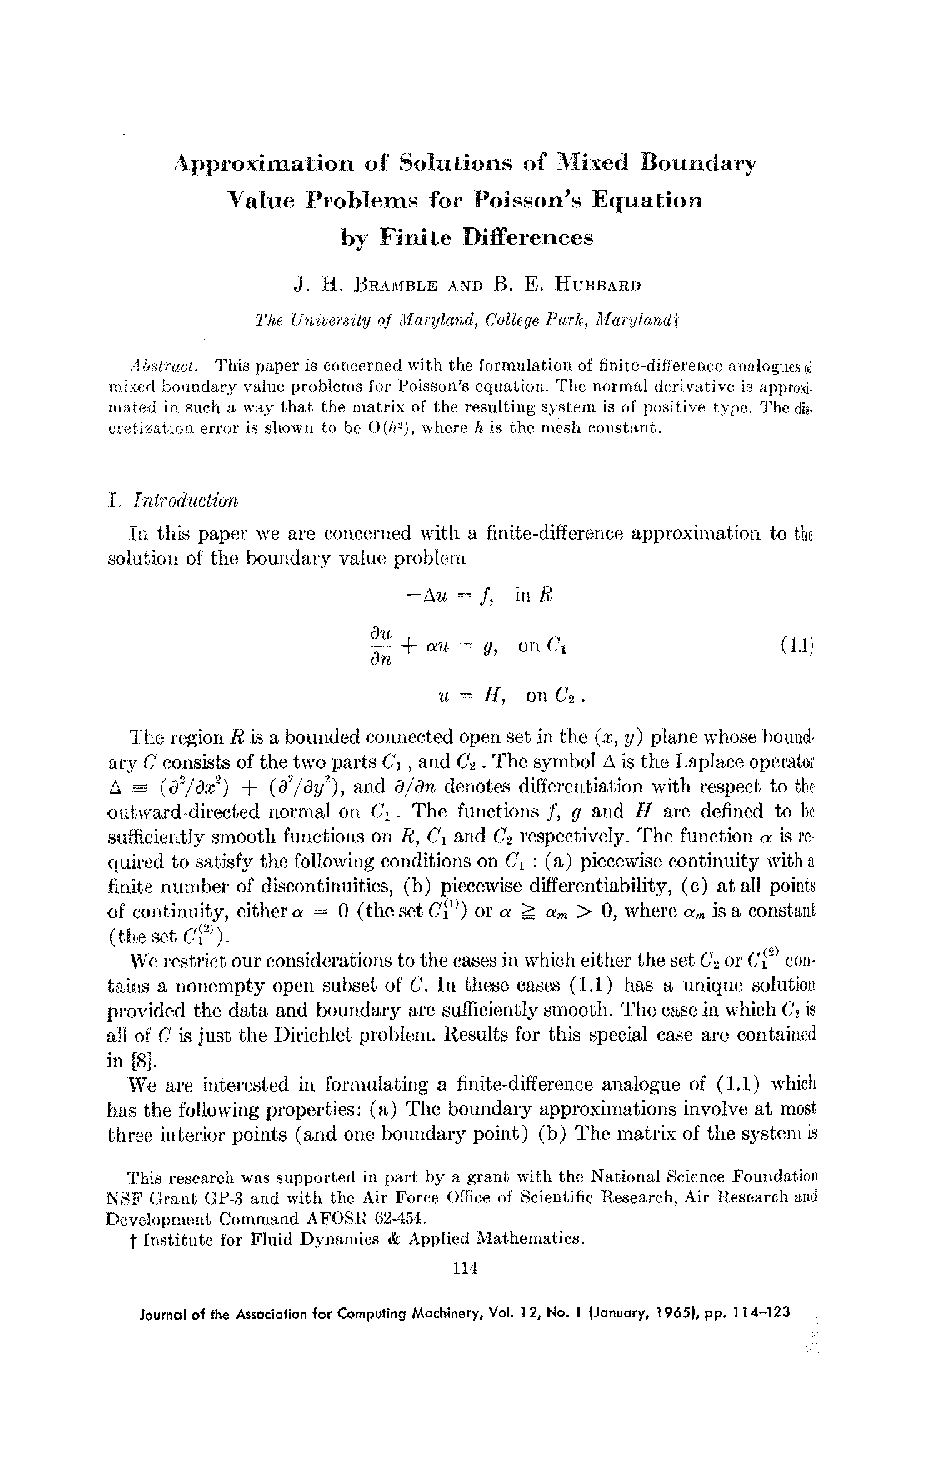
\includepdf[pages = -]{Papers/FDM/bramble1965approximation.pdf}

\section{A finite difference analog of the Neumann problem for Poisson's equation (1965)}
A finite difference analog of the Neumann problem for Poisson's equation \cite{bramble1965finite}

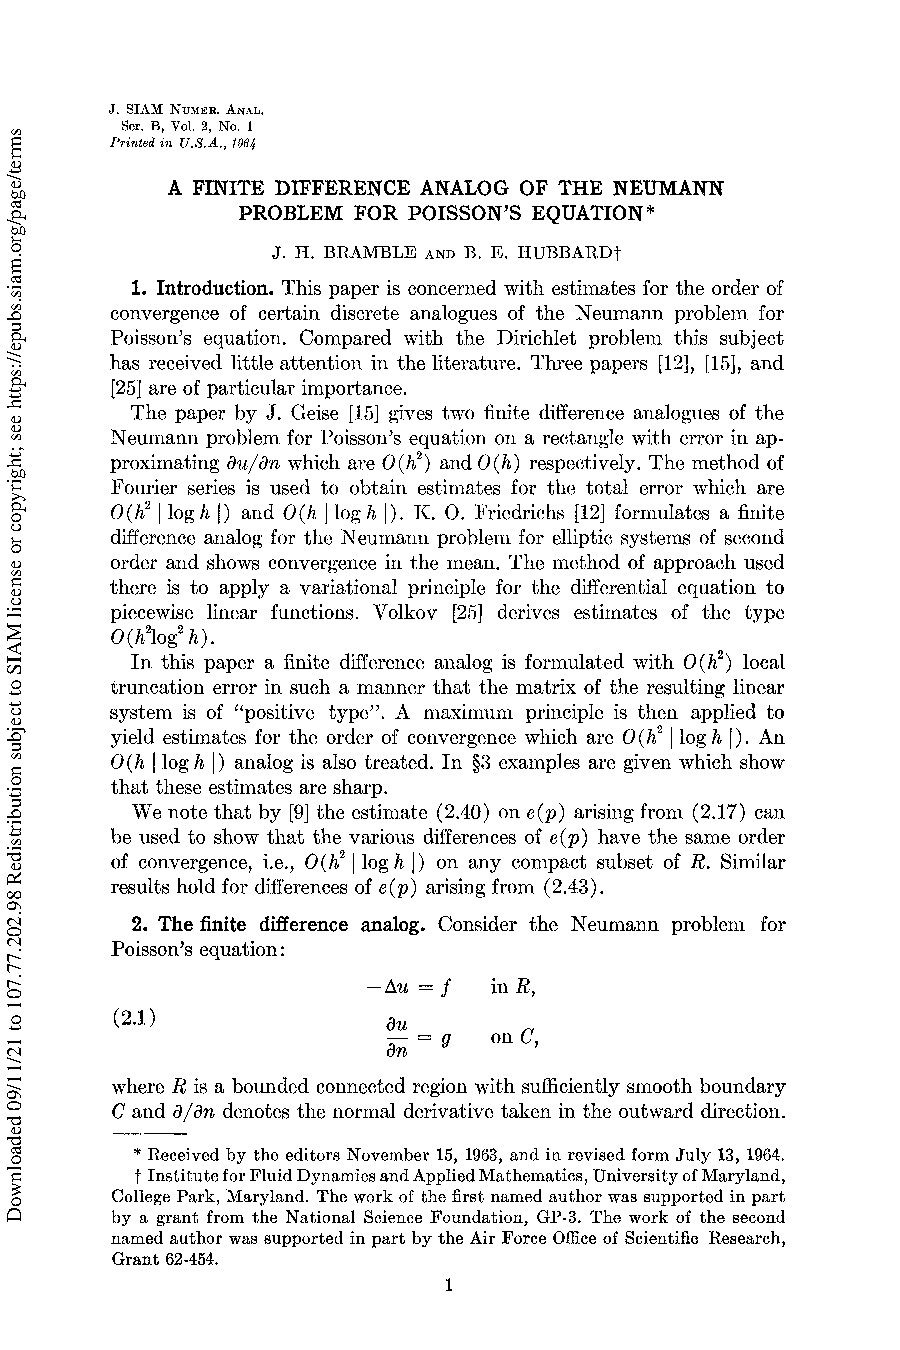
\includepdf[pages = -]{Papers/FDM/bramble1965finite.pdf}

\section{A second order finite difference analog of the first biharmonic boundary value problem (1966)}
A second order finite difference analog of the first biharmonic boundary value problem \cite{bramble1966second}
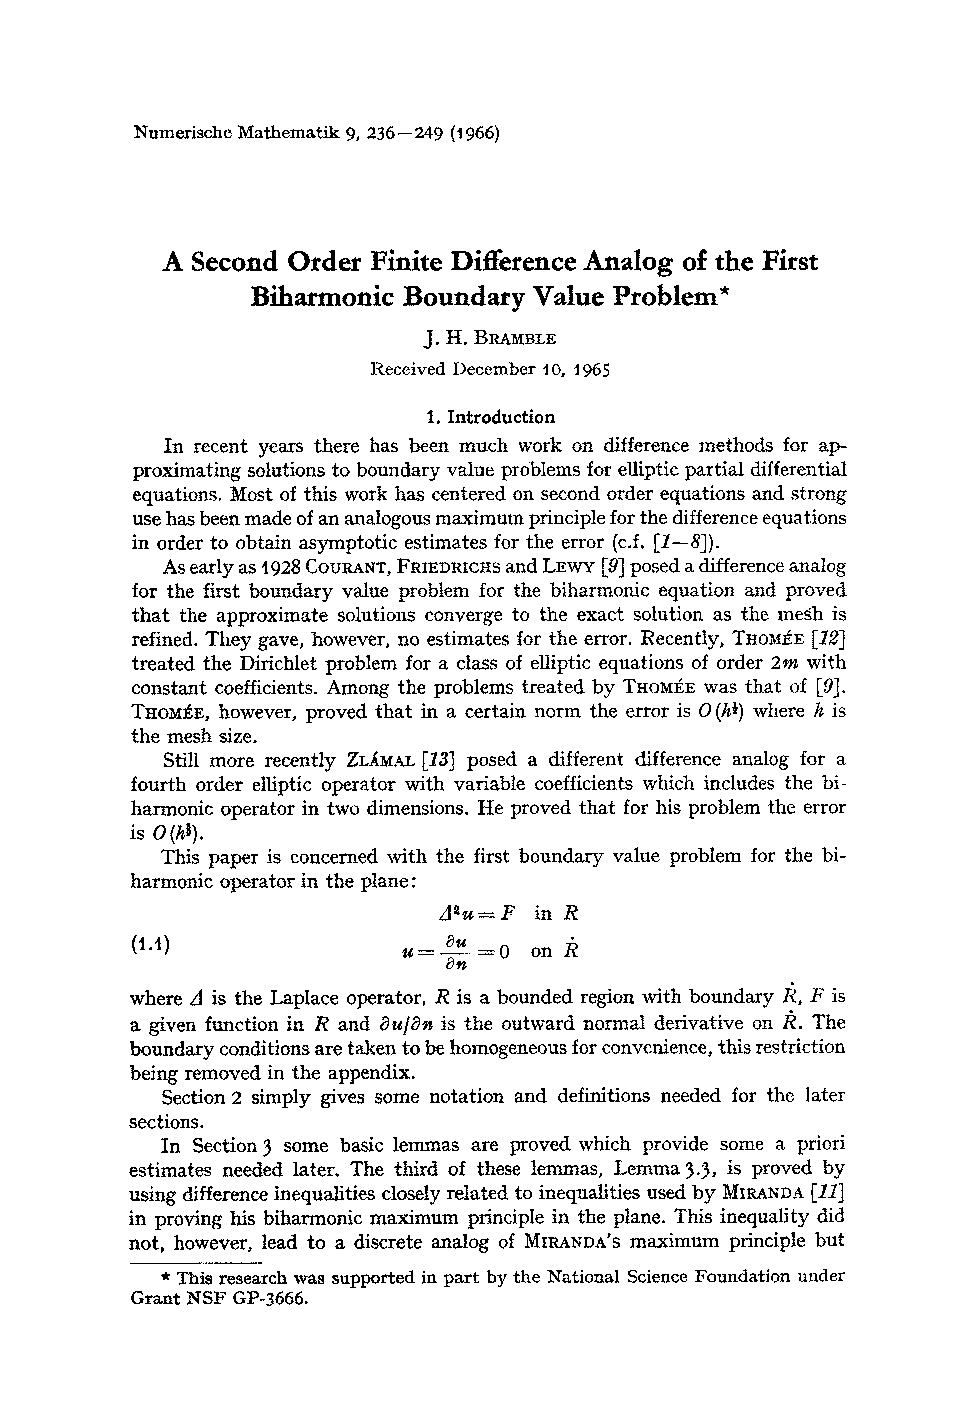
\includepdf[pages = -]{Papers/FDM/bramble1966second.pdf}

\section{Error estimates for difference methods in forced vibration problems (1966)}
Error estimates for difference methods in forced vibration problems \cite{bramble1966error}
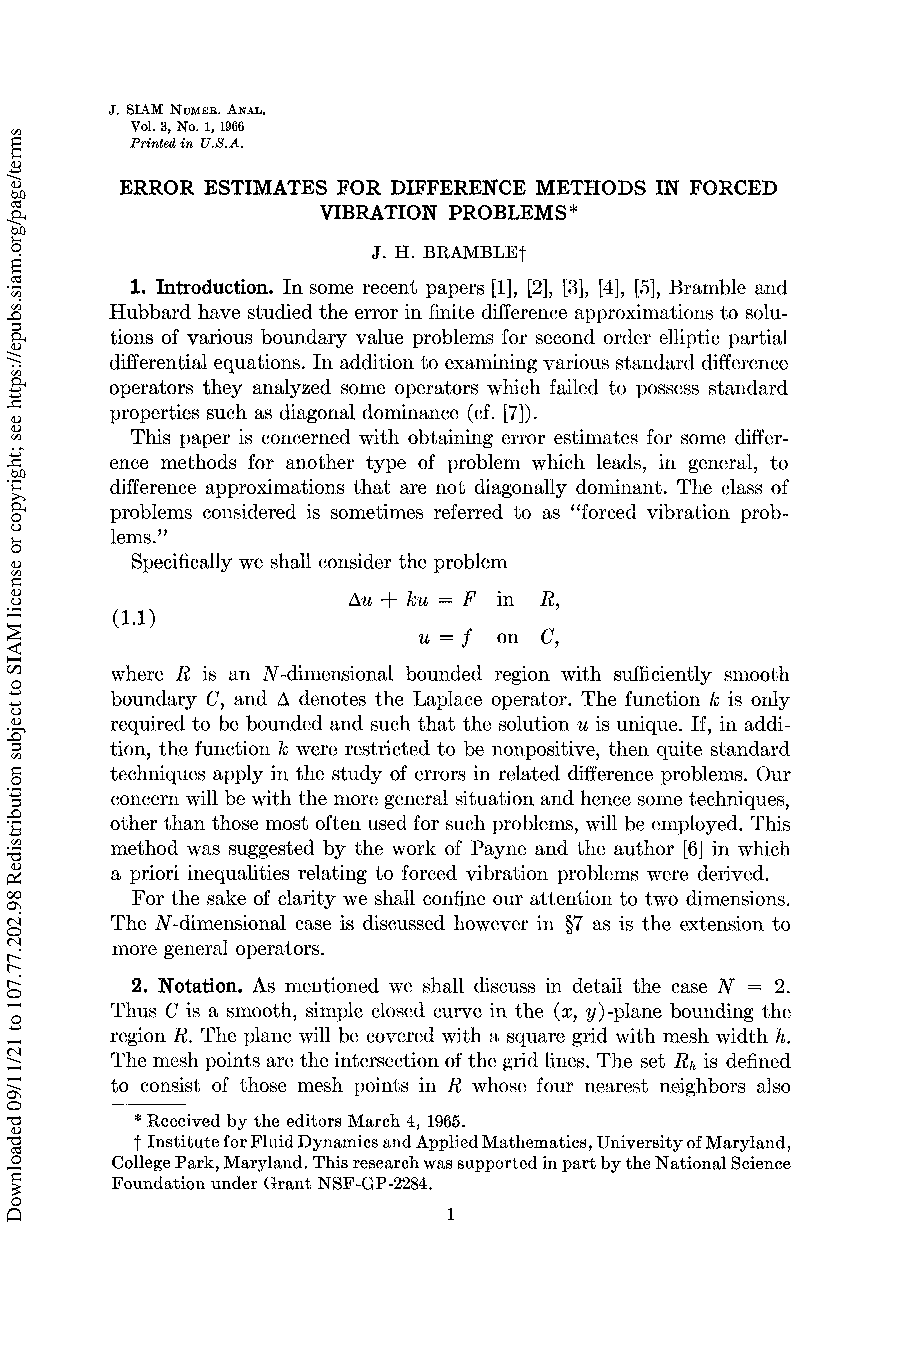
\includepdf[pages = -]{Papers/FDM/bramble1966error.pdf}

\section{On the convergence of difference approximations to weak solutions of Dirichlet's problem (1969)}
On the convergence of difference approximations to weak solutions of Dirichlet's problem \cite{bramble1969convergence}
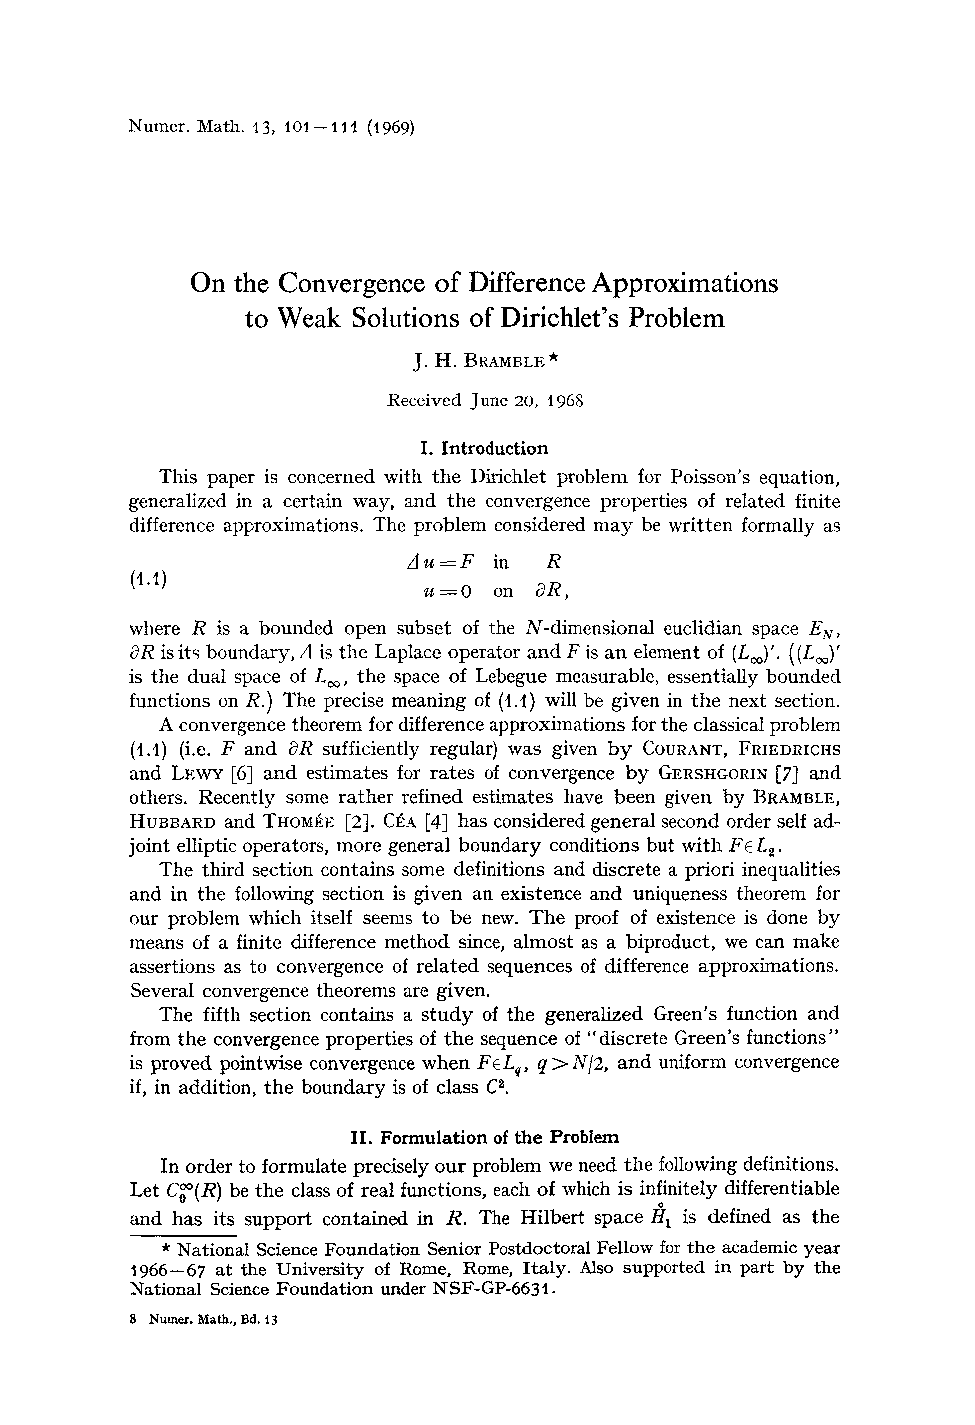
\includepdf[pages = -]{Papers/FDM/bramble1969convergence.pdf}

\subsection{Finite element method}
In the ensuing decades, one of the major focus of Bramble research is on the development and analysis of the finite element method for the approximation of solutions of elliptic and parabolic partial differential equations.


he focused on the numerical analysis of finite element methods.

He had been interested in the development of the theoretical foundation of finite-element methods 

\subsubsection{Bramble-Hilbert lemma}

A collaboration with one of his doctoral students, Stephen Hilbert, resulted in the Bramble-Hilbert Lemma, a theoretical tool for proving error estimates for the finite element method.

One of his most famous result, the Bramble-Hilbert Lemma, was a collaborative effort with his PhD student, Stephen Hilbert \eqref{bramble1970estimation}.

The Bramble-Hilbert Lemma states that for any bounded functional $F:W^{m,p}(\Omega)\mapsto\mathbb R$ that annihilates polynomials of degrees $m-1$, then $F(v)\le C|v|_{m,p,\Omega}$ for any $v\in W^{m,p}(\Omega)$.  What is equally important, as demonstrated in the original paper \eqref{bramble1970estimation}, is how this Lemma is used together with a scaling argument to derivate error estimates for finite element, namely piecewise, 
in terms of Sobolev spaces.  This gives a very general and very elegant way to derive error estimates for piecewise polynomial approximation, for numerical quadratures and many other applications.  It is a basic tool for finite element error analysis and used by every researcher in this field. 


\subsubsection{Post-process and super-convergence}
% Limin will write something
\cite{bramble1989local} presents a general simple post-processing technique for mixed finite element approximations. This technique works for mixed finite element methods as long as there holds a superclose property of the finite element solution.

\cite{bramble1977higher} proposes a local superconvergence result for a large class of Ritz-Galerkin methods solving elliptic boundary value problems. The proposed scheme constructs a better approximation to the solution by employing a convolutional operator. To be specific, the scheme improves the accuracy from $\mathcal{O}(h^r)$ to $\mathcal{O}(h^{2r-2})$ for $r\ge 3$. This convolutional operator does not depend on the specific elliptic operator and is easily constructed.

\subsection{Domain decomposition methods}
Domain decomposition method can be, roughly speaking, divided into two different classes: (1) non-overlapping domain decomposition method, and (2) overlapping domain decomposition method.  In both classes of methods, Bramble has made fundamental contributions

\subsubsection{Non-overlapping domain decomposition methods}
In the sequence of 4 papers \eqref{bramble1986construction, bramble1987construction, bramble1988construction, bramble1989construction}, Bramble, Pasciak and Schatz gave a systematic development of basic non-overlapping domain decomposition methods and the condition number of estimate of the resulting preconditioned systems. 

\subsubsection{Overlapping domain decomposition methods}
Overlapping domain decomposition method can be traced back to Schwarz \eqref{} for two subdomain case and in his original paper, Schwarz also provided a convergence analysis using maximum principle (???).  In ???, Lions used a variational approach to give a convergence analysis in the context of Sobolev space $H^1$ for the two-subdomain case.

In \eqref{brabmel1991convergence}, the first optimal convergence analysis is given for the overlapping domain decomposition methods with coarse space. 

\subsection{Multigrid method}
Multigrid method can be traced back to ????.  A. Brandt has been a major advocate of multigrid method.  Bank and Dupont provided the uniform convergence analysis for multigrid method for 2nd order elliptic boundary value problems. 

Hackbusch and his collaborators set up the mathematical foundation 


\paragraph{The multigrid book}  While Bramble wrote many seminar papers, he wrote very few books. 

He wrote a book “Multigrid Methods”. Multigrid methods are among the most efficient iterative methods for the solution of linear systems which arise in many large scale scientific calculations. Every researcher working with the numerical solution of partial differential equations should at least be familiar with this powerful technique. This invaluable book presents results concerning the rates of convergence of multigrid iterations.

\bibliographystyle{plain}
\bibliography{Bramble.bib}

\end{CJK*}
\end{document}

\section{To Do List}

\begin{enumerate}
\item Selina find some photos in Google
\item Selina:  ask Jenny helps find some old photos 
\item Jinchao finds some newer photos
\end{enumerate} 

\begin{enumerate}
\item Jiang Li, Hong Qingguo and Xu Xiaofeng  论文集

\item Special Issue in Mathematics of Computation
(Ma Limin) 
\item Chen Long:  update Bramble’s Wiki 
\end{enumerate}







